\documentclass{amsart}
\pdfoutput=1
\usepackage{amsmath}
\usepackage{graphicx}
\usepackage{placeins}
\usepackage{amsthm}
\usepackage{nicefrac}
\usepackage{bbm}
\usepackage{wrapfig}
\usepackage{amssymb}
\usepackage{mathrsfs}
\usepackage{fullpage}
\usepackage{color}
\usepackage{makecell}
\usepackage{pifont}
\newtheorem{thm}{Theorem}
\newtheorem{cor}{Corollary}
\newtheorem{lem}{Lemma}
\theoremstyle{definition}
\newtheorem{defn}{Definition}
\DeclareMathOperator{\tr}{Tr}
\DeclareMathOperator{\supp}{supp}
\DeclareMathOperator*{\argmax}{arg\max} % thin space, limits underneath in displays
\newcommand{\ket}[1]{{\left\vert{#1}\right\rangle}}
\newcommand{\bra}[1]{{\left\langle{#1}\right\vert}}
\newcommand{\braket}[2]{{\left< {#1} \middle\vert {#2}\right>}}
\newcommand{\ketbra}[1]{{\left\vert {#1}\middle\rangle\middle\langle{#1}\right\vert}}
\newcommand{\sprod}[2]{\left|\left< {#1} \middle| {#2} \right>\right|}
\newcommand*\dif{\mathop{}\!\mathrm{d}}
\makeatletter
\renewcommand*{\@textcolor}[3]{%
  \protect\leavevmode
  \begingroup
    \color#1{#2}#3%
  \endgroup
}
\makeatother

\interfootnotelinepenalty=10000


\begin{document}
\title{Alternative metrics for contextuality}
\author{Andrew W. Simmons}
\address{Department of Physics, Imperial College London, SW7 2AZ.}
\begin{abstract}
Lorem ipsum dolor sit amet, consectetur adipiscing elit. Fusce laoreet justo porttitor quam euismod consequat. Morbi dapibus lectus at nulla eleifend tincidunt. Mauris vulputate lorem congue sapien tempor bibendum. Fusce risus nunc, dapibus ut tortor sit amet, convallis vulputate magna. Aenean fringilla tincidunt odio, ut pharetra erat aliquam et. Nulla ultrices in odio at rutrum. Morbi vel libero erat. Proin arcu lacus, dignissim et semper malesuada, accumsan id tellus. Duis non ex est. Aliquam lacinia, ex eu hendrerit fermentum, diam nunc sagittis justo, sollicitudin suscipit elit est ut nibh. Ut ac odio nulla.
\end{abstract}
\maketitle
\section{Proofs of Bell-Kochen-Specker Contextuality}

Historically, proofs of Bell-Kochen-Specker, or Maximal, contextuality have tended to have a ``lynchpin" quality; removal of any part of their structure causes the proof to fall apart in its entirety.  In fact, this fact has been exploited in order to tame the maximal contextuality demonstrated by the Peres-Mermin magic square for all qubit states \cite{Berm2016}, as we need only remove the ability to measure one context before it fails to be a proof of contextuality at all. We can think of these structures as exhibiting a kind of circular dependency.

We first need to define what we mean by different strengths of contextuality, following Abramsky and Brandenburger \cite{Abra2011}, as applied to this situation.

\begin{defn}[Hardy Contextuality]
A collection of quantum measurement operators demonstrate \emph{Hardy contextuality} if there is a possible outcome that cannot be explained within a noncontextual, outcome-deterministic ontological model without that model also predicting that some outcomes are possible when they should be impossible.
\end{defn}

\begin{defn}[Maximal Contextuality]
A collection of quantum measurement operators demonstrate \emph{maximal contextuality} if the existence of any noncontextual, outcome-deterministic ontic state in an ontological model for that situation would predict events being possible that should be impossible. %Wow that's a shit definition%.
\end{defn}



Let us consider the 33-ray proof of the Bell-Kochen-Specker theorem due to Peres \cite{Pere1991}. Removing any one context from the structure, \emph{i.e.} not allowing, by some restriction, one basis to be commensurable, also removes all its contextuality. Is this surprising? It seems likely that Peres would deliberately have chosen a minimal example, that could not have anything taken away from it whilst still forming a proof of contextuality, which is a fair comment. However, removing a single context not only renders the structure unable to exhibit maximal contextuality, but \emph{renders it unable to exhibit Hardy contextuality as well}.

That is to say, without introducting other structure to our consideration, we cannot think of this proof of noncontextuality as being a composite of proofs that each possibility is not noncontextually explainable\footnote{If we convert this proof into a proof of nonlocality (which is by nature, state-dependent rather than state-independent), then we can use the structure this gives us to prove something of this form. In this situation, we end up mostly %check%
discarding parts of the restrictions stemming from relationships that exist between contexts rather than removing contexts themselves, in a way which retains operational significance. This is not possible in the contextuality scenario.}. There is no proper subset of the allowable contexts that would constitute a proof that any of its possibilities were contextual. This is somewhat surprising, since we might have expected some contextuality to remain in the system when we introduce a minor epistemic restriction-- the inability to measure one of the sixteen contexts that are quantum-mechanically available in the situation. This ``lynchpin'' property of the scenario can be thought of as reflecting the fact that the distribution is very close to noncontextual in the sense outlined by Winter \cite{Wint2014}. Only one context need be disrupted before the remainder has a classical explanation.

By taking $n$ rotated copies the vectors used in Peres's proof, we can construct a noncontextuality scenario in which $\nicefrac{n}{33}$ of the contexts need to be disrupted in order for the statistics to be explained noncontextually.

In this paper, we will investigate how we can use these ideas as alternative metrics for the contextuality displayed by a particular operational scenario, with a focus on possibilistic cases. First, we will consider the case of nonlocality, and demonstrate hardness results for computing how nonlocal, given this definition, a no-signalling scenario is. Then, moving to the more general contextuality scenario, we will investigate within a graph-theoretic framework how robust, in this sense, different Kochen-Specker sets are; and set a bound on how robust any quantum scenario can be. We will demonstrate that it is possible that other physical theories can be more contextual, given this definition, than quantum mechanics. We can consider this as a stronger analogue than the observation that a PR-box is more nonlocal with respect to the CHSH inequality than any quantum-mechanically accessible scenario.



\section{Alternative definitions of contextuality as contextuality measures}

One metric for contextuality that has appeared in the literature \cite{Abra2011, DeSi2015}, is the \emph{contextual fraction}, in which we consider our probability distribution to be a convex mixture between a noncontextual theory and a contextual one. This notion is what prompts the term ``maximal contextuality''; if a scenario is maximally contextual then it has a contextual fraction that is the highest possible: 1. Other metrics have also been explored; one important one, possessing operational meaning, is \emph{negativity} (find cite). These definitions have their own strengths and weaknesses. Both are independent of re-labelling the measurement effects, but contextual fraction has no apparent operational relevance, and negativity is defined relative to a specific choice of frame, with no known procedure for its minimisation.

Let us consider the case of nonlocality. Operationally, our scenario is represented by some sort of data table, such as the one below:

\begin{equation}\renewcommand{\arraystretch}{1.5}
\begin{array}{c| c c | c c |} \renewcommand{\arraystretch}{1.5}
&\ket{+}&\ket{-}&\ket{0}&\ket{1}\\\hline
\ket{+}&\frac{3}{4} &\frac{1}{12}  &\frac{2}{3} & \frac{1}{6}\\
\ket{-}&\frac{1}{12} &\frac{1}{12}  &0 &\frac{1}{6}\\ \hline
\ket{0}&\frac{2}{3}&0&\frac{1}{3} &\frac{1}{3} \\
\ket{1}&\frac{1}{6}&\frac{1}{6} &\frac{1}{3} &0 \\ \hline
\end{array} \renewcommand{\arraystretch}{1}
\end{equation}
This is a table of probability outcomes for a nonlocality experiment on the state $\nicefrac{1}{\sqrt{3}}\left(\ket{00}+\ket{01}+\ket{11}\right)$, and it demonstrates Hardy nonlocality. The $\ket{-}\ket{-}$ outcome possibility cannot be accounted for within a local hidden variable model; and such this model has a \emph{paradoxical probability}, the maximum probability over contexts of exhibiting a nonlocal possibility, of $\nicefrac{1}{12}$. The maximum for any Hardy paradox, a table exhibiting these exact possibilities, is given by $\nicefrac{5\sqrt{5}-11}{2}$. (This nonlocal possibility is also sometimes called the EPR2 decomposition).

We see that this scenario, then, has a nonlocal fraction strictly greater than the paradoxical probability; were we able to find a data table corresponding to a deterministic hidden variable, and subtract it from the given data table in a way that respected no-signalling and accounted for the probability of the nonlocal possibility, then the possibility would not be nonlocal in the first place!
Calculation of the contextual fraction is computationally complex; indeed, determining whether it is nonzero is \textsc{NP-complete} for a 
nontrivial two-party nonlocality scenario exactly when one party has access to measurements with three or more outcomes \cite{SimmCC}.

We can define operationally-motivated metrics for nonlocality based on the variational distance between a given probability distribution and its closest local distribution, broken down into comparable contexts. For example, we could define the distance as being the statistical distinguishability of the distribution from the nearest local distribution, taking an average or a maximum over contexts. These correspond to operational situations where we pick contexts at random, and seek to distinguish the two distributions, or where we are allowed to choose a context in which the distributions are maximally different.

\begin{equation}
\delta_{\mbox{av}}(\mathcal{P})=\sup_{\mathcal{L}\in\mathscr{L}}\delta_1(\mathcal{P},\mathcal{L})=\frac{1}{2\left|\mathcal{C}\right|}\sup_{\mathcal{L}\in\mathscr{L}}\sum_{C\in\mathcal{C}}\sum_{x\in C}\left|\mathcal{P}(x)-\mathcal{L}(x)\right|
\end{equation}

\begin{equation}
\delta_{\mbox{max}}(\mathcal{P})=\sup_{\mathcal{L}\in\mathscr{L}}\delta_2(\mathcal{P},\mathcal{L})=\frac{1}{2}\sup_{\mathcal{L}\in\mathscr{L}}\max_{C\in\mathcal{C}}\sum_{x\in C}\left|\mathcal{P}(x)-\mathcal{Q}(x)\right|
\end{equation}

For instance, the Hardy distribution shown above has the following distribution as its closest local distribution, no matter whether we take the maximal variation distance or average it over contexts:

\begin{equation}\renewcommand{\arraystretch}{1.5}
\begin{array}{c| c c | c c |} 
&&&&\\\hline
&\frac{3}{4} &\frac{1}{8}  &\frac{2}{3} & \frac{5}{24}\\
&\frac{1}{12} &\frac{1}{24}  &0 &\frac{1}{8}\\ \hline
&\frac{2}{3}&\frac{1}{24}&\frac{3}{8} &\frac{1}{3} \\
&\frac{1}{6}&\frac{1}{8} &\frac{7}{24} &0 \\ \hline
\end{array} \renewcommand{\arraystretch}{1}
\end{equation}
This gives rise to a distinguishability from local distributions of $\nicefrac{1}{24}$.
These are sensible metrics for nonlocality. In particular, they have the following properties:

\begin{thm}
Both the average variation distance and maximum variation distance posess the following desirable properties for a nonlocality metric:
\begin{enumerate} 
\item They are non-increasing under local classical post-processing.
\item They are constant under re-labelling of outcomes or outcome coarse-graining. This follows from basic statistics. Clearly two distributions can't be more distinguishable if we throw away information.
\item They are linear under mixing with local distributions. Clearly obvious.
\end{enumerate}
\end{thm}

\begin{proof}
Do this later i guess.

\end{proof}

Note: nonlocality metrics are very well-studied. This must be coincident with something. maybe it's coincident with "maximum violation of a Bell inequality". It's sort of related to nonlocal fraction but as we have pointed out it can't be identical to it. "Robustness measure of nonlocality" often distance when mixing with pure noise.

\section{Possibilistic Measures of Nonlocality}

The sheaf-theoretic approach to nonlocality introduces the concept of "logical" contextuality/nonlocality by considering probability theories in semirings other than $\mathbb{R}_+$, for example the Boolean semiring. Doing so restores the concept of nonlocality as being defined by the violation of inequalities corresponding to facets of a local polytope. However, this setting poses a mathematical problem for our scheme: without additive inverses, we cannot proceed with our definitions as written. We also do not have access to division, which rules out other statistical distance measures such as the Kullback-Liebler divergence.

Given that our semiring may not be extendable into a ring, in this case we must define our statistical distances relative to some penalty function that obeys the following properties:

blehhh

Proofs of maximal contextuality can be converted into proofs of maximal nonlocality by obvious thing. Can then talk about distance from local polytope as sensible measure. Same of Hardy contextuality and Hardy nonlocality.
What does this end up meaning? Is this identical to the description by Winter?

We saw that for a contextuality situation, a measure of the strength of a maximal contextuality scenario was the number of projectors whose values needed to depend on context . For a nonlocality scenario (which is of course inherently state-dependent), we have a choices in how we interpret this condition. We could count the minimum number of maximally-fine grained projectors whose outcomes depend on context, so if Alice measures in the basis $\{\ket{a_0},\ket{a_1}\dots\ket{a_n}\}$, and Bob measures in the basis $\{\ket{b_0},\ket{b_1}\dots\ket{b_n}\}$, we are counting projectors of the form $\ket{a_i}\ket{b_j}$ which have context-dependent outcomes. However, in many nonlocality scenarios, each of these fine-grained projectors may only occur in a single context, and so while this is the most obvious analogue to the maximal contextuality scenario described above, this metric does not capture the structure of the nonlocality problem.

Perhaps a more fruitful approach is to consider how many of the projective measurements available to a single party must be found to have outcomes that depend on the context of which measurement choice is chosen by the other partner. A different generalisation is that we could count the minimum number of contexts that can deviate in their outcomes from a specified set of global valuations. We shall see that both of these are valid measures of possibilistic nonlocality, but have very differing properties with respect to how much nonlocality can be considered achievable by quantum mechanics, as well as the computational complexity of calculating each value.

\begin{defn}[$k$-\textsc{PN1}]
We define the decision problem $k$-\textsc{PN1} as follows; the input is a table of data as in \cite{Mans2011} and an integer $k$, and we ask the following question: is there an explanation of the table in which the number of projectors available to the two parties whose outcomes depend on context is less than or equal to $k$.
\end{defn}
\begin{thm}$k$-\textsc{PN1} is \textbf{NP}-complete when each party's measurements have exactly two outcomes.
\end{thm}

\begin{proof}
The proof will be by reduction from \textsc{Vertex Cover}, whose definition, as given by Garey and Johnson \cite{Gare1979}, is as follows:
\begin{defn}[\textsc{Vertex Cover}]
\quad\\
Instance: a graph $\mathcal{G}=(V,E)$ and a positive integer $k\leq V$.\\
Question: is there a $V'\subset V$ such that $\left|V'\right|\leq k$ and for all $e\in E$, $V\cap e\neq\emptyset$.
\end{defn}

We will now construct a nonlocality scenario from a given instance of \textsc{Vertex Cover} such that there exists a vertex cover for $\mathcal{G}$ of size $k$ if and only if there exists an explanation of the nonlocality scenario in which the number of projectors with context-independent valuation is $k$. %+\left|E\right|

 Each of the four contexts that makes up the Hardy paradox will have criteria that must be met by a set of contextual rows and columns to be able to explain the paradox. For the context containing the 1 entry that cannot be extended to a deterministic grid, the sufficient conditions are always satisfied by one of the following: ``the measurement row must be contextual", ``the measurement column must be contextual", or ``the measurement row and column must be contextual". The remaining contexts can always be satisfied by \emph{either} one of the following:``the measurement row must be contextual", or ``the measurement column must be contextual". We never require both the measurement column and row to vary, as this would be a violation of no-signalling.

Given a graph $\mathcal{G}=(V,E)$, we construct a nonlocality scenario in which there are $2\left|E\right|$ measurement rows and $\left|V\right|$ measurement columns, noting that since there are only $O(\left|V\right|^2)$ possible edges. Let us label the edges $e_i=\{v^i_1,v^i_2\}$, and for each edge, we place a Hardy paradox in the contexts at the intersections of the measurement rows labelled $2i$ and $2i+1$, and the measurement columns $v^i_1$, and $v^i_2$. Every other context should contain all 1-entries. The Hardy paradoxes we have placed may not be the only Hardy paradoxes in the scenario, due to ``interactions'' between the paradoxes that share measurement rows. %How important is this?

Assume there is a vertex cover for $\mathcal{G}$ of size $k$, namely $K=\{v^K_1,v^K_2\dots v^K_k\}$, and then consider an explanation for the nonlocality scenario in which measurement columns indexed by $K$ are allowed to have outcomes that vary contextually. We will now show that this is a sufficient explanation for the nonlocality scenario.

% Insert proof here but it's basically obvious

We note that for such a scenario, a $k$ minimal for the graph is also a $k$ minimal for the nonlocality scenario: allowing any measurement row to vary contextually affects exactly one of the Hardy paradoxes introduced deliberately by the graph structure, while allowing a measurement column to vary contextually affects affects strictly more than one. Hence, if in a given explanation of the nonlocality scenario, there is a measurement row with a context-dependent outcome, we can replace it with one of the columns involved in the Hardy paradox that involves contexts on that row. By iterating this, we are left with an explanation in which only measurement columns, not rows, are required to vary contextually, which, by construction, is exactly a vertex cover for $\mathcal{G}$. Hence, the size of a minimal vertex cover for $\mathcal{G}$ and the minimal explanation for the nonlocality scenario are equal.

We have exhibited a polynomial-time reduction from \textsc{Vertex Cover} to $k$-\textsc{PN1}. Since  \textsc{Vertex Cover} is \textbf{NP}-hard, so too, then, is $k$-\textsc{PN1}.  In addition, $k$-\textsc{PN1} is in \textbf{NP} since there are only polynomially many 1 entries in the grid and therefore a witness that is an explicit set of data tables that combine to the target table is of polynomial size.
\end{proof}
By this reduction from \textsc{Vertex Cover}, we find that unless \textbf{P}=\textbf{NP}, $k$-\textsc{PN1} is not approximable in polynomial time to a factor of better than 1.3606 \cite{Dinu04}, or better than 2 if the Unique Games conjecture holds \cite{Khot03}.

The cases in which one party has a number of measurements greater than two can be seen to be \textbf{NP}-hard since they are already \textbf{NP}-hard for $k=0$ \cite{Abra2011,SimmCC}. This demonstrates another sense in which the case treated by Mansfield and Fritz \cite{Mans2011,Mans2016} is unique.



\begin{defn}[$k$-\textsc{PN2}]
We define the decision problem $k$-\textsc{PN2} as follows; the input is a table of data as in \cite{Mans2011} and an integer $k$, and we ask the following question: is there an explanation of the table in which the number of contexts in which outcomes are allowed to freely vary is less than or equal to $k$.
\end{defn}
\begin{thm}$k$-\textsc{PN2} is \textbf{NP}-complete when each party's measurements have exactly two outcomes.
\end{thm}
\begin{proof}
The proof will proceed once again by reuction from \textsc{Vertex Cover}. Like in the constructions of Abramsky, Gottlob, and Kolaitis, we will in this instance use a data table that is symmetric on exchange of columns and rows.

Given a graph, 
Given a graph $\mathcal{G}=(V,E)$, we construct a nonlocality scenario in which there are $\left|V\right|$ measurement rows and columns. Each context at the intersection of the $n$\textsuperscript{th} measurement row and $n$\textsuperscript{th} measurement column is defined to be
\begin{equation}
\begin{array}{| c c |} 
\hline
 1& 1\\ 
 1 & 0\\ \hline
\end{array}\,,
\end{equation}
which we will refer to as a ``type '' context.
For each edge, $e=\{v_1,v_2\}\in E$, we will define contexts located at the intersection of the $v_1$\textsuperscript{th} measurement row and the $v_2$\textsuperscript{th} measurement column and at the intersection of the $v_2$\textsuperscript{th} measurement row and the $v_1$\textsuperscript{th} measurement column to be
\begin{equation}
\begin{array}{| c c |} 
\hline
 0& 1\\ 
 1 & 1\\ \hline
\end{array}\,,
\end{equation}
which we will refer to as a ``type 2'' context. The remaining contexts will be 
\begin{equation}
\begin{array}{| c c |} 
\hline
 1& 1\\ 
 1 & 1\\ \hline
\end{array}\,,
\end{equation}
a ``type 0'' context. We note that for each edge $\{v_1,v_2\}$, we introduce four Hardy paradoxes, each involving the four contexts at $(v_1,v_1)$, $(v_1,v_2)$, $(v_2,v_1)$ and $(v_2,v_2)$. The nonlocal 1 entries are shown here in red:
\begin{equation}
\begin{array}{| c c |c c|} 
\hline
 \textcolor{red}{1}& 1&0&1\\ 
 1 & 0&1& \textcolor{red}{1}\\ \hline
 0& 1& \textcolor{red}{1}&1\\ 
 1 & \textcolor{red}{1}&1&0\\ \hline
\end{array}\,.
\end{equation}
A Hardy paradox can only be formed when one of the following structures appears in a square pattern:


Proof unfinished- this proof technique may not work


\end{proof}

\section{How robust can quantum maximal contextuality be?}

Consider the orthogonality graph $\mathcal{G}$ of a maximal nonlocality scenario, in which we identify projectors with vertices, and two vertices $g_1$, $g_2$, identified with $\ket{\psi_1}$, $\ket{\psi_2}$ are joined by an edge iff $\braket{\psi_1}{\psi_2}=0$. Following Renner and Wolf \cite{Renn2004}, we will restrict our attention to outcome assignments in which we do not ever assign a ``1'' valuation to two orthogonal vectors; this is known as a \emph{weak Kochen-Specker set}. A weak Kochen-Specker set can be extended to a full Kochen-Specker set with the addition of $O(|\ket{\psi_i}|^2d)$ extra vectors, or we can consider the incomplete bases as being completed by additional projectors, whose valuations are allowed to be contextual as they are outside the scope of our scenario. An \emph{independent set} is a subset of vertices, none of which are joined by an edge. Any noncontextual assignment of ``1''s, then, will form an independent set since we cannot have two orthogonal vectors, \emph{i.e.} vertices joined by an edge in our set of vectors which are noncontextually given ``1'' assignments. The size of the largest independent set of a graph $\mathcal{G}$ is denoted $\alpha(\mathcal{G})$ and is called the \emph{independence number}. Another important graph concept is that of a clique:%can put some good motivation for this approach here- in most graph-based KS proofs the coarse-grained projectors are effectively allowed to vary contextually in their assignment 

\begin{defn}[Clique]
For a graph $\mathcal{G}=\{V,E\}$, a vertex subset $C\subset V$ is a \emph{Clique} if the subgraph induced from $\mathcal{G}$ on $C$ is \emph{complete}, that is,  every vertex in $C$ is connected to every other.
\end{defn}

We say that a clique is \emph{maximal} if it cannot be extended by including one more vertex, and that it is a \emph{maximum clique} if there is no clique in $\mathcal{G}$ with more vertices. The size of a maximum clique in $\mathcal{G}$ is denoted $\omega(\mathcal{G})$, and so we note that for a $d$-dimensional quantum system, as long as the set of vectors we can measure includes at least one basis, we will have $\omega(\mathcal{G})=d$. In a complete hidden variable model for a scenario, we require that in every context, there be at least one vector that can take a ``1'' value either contextually or noncontextually. This motivates the following definition:



\begin{defn}[Maximum-clique hitting-set]
For a graph $\mathcal{G}=\{V,E\}$, a vertex subset $T\subset V$ is a \emph{maximum-clique hitting-set} or \emph{maximum-clique transversal} if for all cliques $C$, $|C|=\omega(\mathcal{G})$, $T\cap C\neq\emptyset$.
\end{defn}

Clearly, the set of vertices associated with a set of vectors given either noncontextual or contextual ``1'' assignments is a Maximum-clique hitting set. This allows us to define our first figure-of-merit for a set of vectors forming a Kochen-Specker type proof of the Bell-Kochen-Specker theorem.

\begin{equation}q_a(\mathcal{G})=\min_T \min_{A\subset T} |T|-|A|\end{equation},
where $T$ is a maximum-clique hitting-set. We see that this is a graph-theoretic representation of the possibilistic figure-of-merit we posited above: we take a set $T$ of vectors which will recieve a ``1'' valuation, either contextually or noncontextually, and subtract from it the number of those vectors that can support a noncontextual valuation. It is therefore the number of vectors that must recieve a contextual valuation in any model for the scenario. However, we can note that it is possible to achieve an arbitrarily high value of $q_a$ just by taking an equal number of noninteracting copies of, for example, the Peres-Mermin magic square. In order that we might more directly compare this quantity between graphs of different sizes, we can consider its graph density:
\begin{equation}
q(\mathcal{G})=\frac{q_a(\mathcal{G})}{|V(\mathcal{G})|}.
\end{equation}
We now have a graph-theoretic formulation of our quantity of interest. What values of this quantity are obtainable, either by quantum-mechanically realisable scenarios, or in general probabilistic theories? We note the following trivial lower bound:
\begin{equation}
q_a(\mathcal{G})\geq \min |T|-\alpha(\mathcal{G}).
\end{equation}
We note that in general, it is \textbf{NP}-complete to calculate the value of $\min |T|$ if we know $\omega(\mathcal{G})$, since for triangle-free graphs, this is equivalent to finding a vertex cover, which is \textbf{NP}-complete \cite{Polj1974}. Also, it is \textbf{NP}-complete to calculate $\alpha(\mathcal{G})$ \cite{Gare1979}. 

We will now demonstrate an upper bound on the quantity $q(\mathcal{G})$ for any quantum-mechanically accessible $\mathcal{G}$ in terms of the quantum dimension of the vectors that give rise to it.
\begin{thm}
Any orthogonality graph $\mathcal{G}$ induced by a set of vectors $\ket{\psi_i}$ in a $d$-dimensional Hilbert space has
\begin{equation}
q(\mathcal{G}) \leq \left(1-\frac1d\right)^{d-1}-\frac{1}{2^{d-1}}.
\end{equation}
\end{thm}
\begin{proof}
The proof proceeds by demonstrating the existence of a region of Hilbert space, such that any basis for that Hilbert space must have at least one basis element that lies within the region, as well as demonstrating a lower
bound on the size of an independent set of vectors within that region.

Consider a basis for $\mathcal{H}_d$. Without loss of generality, we can take this to be the standard basis for the set. By symmetry concerns, the quantity $\min_i \left|\braket{\psi}{i}\right|$ is maximised (albeit nonuniquely) by $\ket{\psi}=d^{\nicefrac{-1}{2}}\sum_i\ket{i}$. This puts an upper bound on the size of the largest hyperspherical angle that can separate an arbitarary vector from its closest basis element. A closed complex hyperspherical cap subtending this angle will then necessarily capture at least one element from the basis, and so any set of vectors within such a hyperspherical cap $C$ construe a maximum-clique hitting-set, $T_C$.

A closed complex hyperspherical cap centered at $\ket{\psi}$ in question can be thought of as the set of vectors $\ket{\phi}\in\mathcal{H}_d$ such that $\sprod{\psi}{\phi}^2\geq t$ for some $t\in\mathbb{R}$. The derivation of the volume of this annulus in $\mathbb{C}^d$ is given in [cite] and we reproduce it here:

\begin{equation}V=\frac{2\pi^n(1-t)^{d-1}}{(d-1)!}\end{equation}
Plugging in $t=0$, we get the volume for the entire hypersphere:
\begin{equation}V_S=\frac{2\pi^n}{(d-1)!}\end{equation}
And so the hyperspherical cap in which we are interested takes up $\nicefrac{V}{V_S}=(1-t)^{d-1}$ of the Hilbert space. Plugging in the value derived above for the necessary $t$ to be sure of capturing at least one element from each basis, we get the value
\begin{equation}
\frac{V}{V_S}=\left(1-\frac1d \right)^{d-1}.
\end{equation}
Clearly, the value of $q(\mathcal{G})$ for a quantum graph is upper bounded by the size of any maximum-clique hitting set, so if we can bound the minimum number of vectors we c must intersect with such a hyperspherical cap, this also constitutes a bound on the value $q(\mathcal{G})$. However, we would not expect this bound to be tight, since we have ignored the independent set subtrahend entirely. We would like to demonstrate an independent set within our maximum-clique hitting-set $T_C$, and therefore give a precise upper bound on the quantity $q_a(\mathcal{G})=\min_T \min_{A\subset T} |T|-|A|$, giving an explicit construction procedure for a $T$ and $A\subset T$.

We note that a hyperspherical cap containing the vectors $\ket{\phi}$ such that $\sprod{\psi}{\phi}^2> \nicefrac12$ cannot contain two orthogonal vectors as a simple application of the triangle inequality. We can place this smaller hyperspherical cap anywhere within the larger hyperspherical cap, and this will form an independent set $A$ that is a subset of $T_C$. For the rest of this proof, we will assume that the two hyperspherical caps are centred on the same point; this will make no difference to the worst case scenario which forms the bound. The region of Hilbert space, then, in which vectors count towards the figure of merit, is a member of a two-parameter family of \emph{annuli} on the complex hypersphere, defined by
\begin{equation}
t_1\leq\sprod{\psi}{\phi}^2< t_2.
\end{equation}
Such an annulus takes up a proportion 
\begin{equation}p(t_1,t_2)=\left(1-t_1 \right)^{d-1}-\left(1-t_2 \right)^{d-1}\end{equation}
of the Hilbert space. Our construction has $t_1=\nicefrac1d$, and $t_2=\nicefrac12$, giving us a hyperspherical annulus defined by
$\nicefrac1d\leq\sprod{\psi}{\phi}^2< \nicefrac12$.
It now remains to be proved that no matter the positions of the set of vectors $\{\psi\}$, there must be some place in which we can place this annulus such that we only intersect strictly less than $p(t_1,t_2)$ of them. 

Consider the canonical action of $SU(d)$ on the unit hypersphere in $\mathbb{C}^d$, which we shall denote $S_\mathbb{C}^d$. We define a space $SU(d)\times S_\mathbb{C}^d$, where $SU(d)$ is equipped with the Haar measure, and $S_\mathbb{C}^d$ is equipped with the uniform measure.

At each $\ket{\psi_i}$, we place a bump function $f^\epsilon_\ket{\psi_i}$ with unit integral and support only within a disc of radius $\epsilon$ around $\ket{\psi_i}$, where $\epsilon$ is taken to be sufficiently small compared to $d$.

Let $A_{t_1,t_2}$ denote the hyperspherical annulus, $\{\ket{\phi}|t_1\leq\sprod{\psi}{\phi}^2< t_2\}$, centred at $\ket{0}$, with a volume $V$ such that $\nicefrac{V}{V_S}=p$. We consider the following quantity:
\begin{equation}
\oint_{SU(d)\times S_\mathbb{C}^d} \mathbbm{1}_{g.z\in A_{t_1,t_2}} \sum_i f_\ket{\psi_i}(z) \dif g\dif z.
\end{equation}
By Fubini's theorem, we have:
\begin{align}
\int_{SU(d)} \oint_{S_\mathbb{C}^d} \mathbbm{1}_{g.z\in A_{t_1,t_2}} \sum_i f^\epsilon_\ket{\psi_i}(z) \dif z \dif g &= \oint_{S_\mathbb{C}^d} \int_{SU(d)}  \mathbbm{1}_{g.z\in A_{t_1,t_2}} \sum_i f^\epsilon_\ket{\psi_i}(z) \dif g \dif z \\
\int_{SU(d)} h(g,p,\epsilon) \dif g  &= \sum_i\oint_{S_\mathbb{C}^d}f^\epsilon_\ket{\psi_i}(z)  \int_{SU(d)} \mathbbm{1}_{g.z\in A_{t_1,t_2}} \dif g \dif z \label{eqn:1} \\
 &= p(t_1,t_2)\sum_i\oint_{S_\mathbb{C}^d}f^\epsilon_\ket{\psi_i}(z)  \dif z \label{eqn:2} \\
&= p(t_1,t_2)\left|\ket{\psi_i}\right|
\end{align}



In which equality holds between equations \ref{eqn:1} and \ref{eqn:2} since as the indicator function for the annulus is twirled by the rotation group it becomes a constant function with value $p(t_1,t_2)$. Now, we would like to interpret the left hand side as an average over the elements $g\in SU(d)$ of $h(g,p,\epsilon)$, the number of the $\ket{\psi_i}$ that intersect the annulus $g^{-1}A_{t_1,t_2}$. However, we note that since the bump functions are not exact delta functions, there is by necessity some over- or under-counting of the point density, depending on whether a bump function, centred inside the annulus, has some of its measure outside the annulus; or a bump function centred outside the annulus has some of its measure within. We note that if we extend our annulus's extent by $\epsilon$, we capture the entirety of the measure of the bump functions inside the original annulus. This means that the expression now represents an overestimate of the exact count of points within the annulus $g^{-1}A_{t_1,t_2}$. Contracting the annulus by $\epsilon$, so that we have $t_1\rightarrow t_1-\epsilon$ and $t_2\rightarrow t_2+\epsilon$,  has an effect on the proportion of the sphere taken up by the annulus:
\begin{align}
p(t_1-\epsilon,t_2+\epsilon)&=\left(1-t_1+\epsilon\right)^{d-1}-\left(1-t_2-\epsilon\right)^{d-1}\\
&=(1-t_1)^{d-1}-(1-t_2)^{d-1}+(d-1)\epsilon\left((1-t_1)^{d-2}+(1-t_2)^{d-2}\right)+o(\epsilon).
\end{align}
We can consider this to be a strict overcount of the true number of points within the annulus. We therefore get, applying the relevant values for $t_1$ and $t_2$,
\begin{align}
q(\mathcal{G})&\leq \lim_{\epsilon\rightarrow0}p(t_1-\epsilon,t_2+\epsilon) \\
&\leq \left(1-\frac1d\right)^{d-1}-\frac{1}{2^{d-1}}.
\end{align}

\end{proof} 
\begin{cor}
Any quantum mechanically accessible $\mathcal{G}$ has  $q(\mathcal{G})\leq\nicefrac{4251920575}{11019960576}\sim0.385838$.
\end{cor}
\begin{proof}
Calculating the derivative of $ \left(1-\frac1d\right)^{d-1}-\frac{1}{2^{d-1}}$ with respect to $d$ shows that it takes a maxmimum between $d=9$ and $d=10$. Evaluation of the quantity at these points reveal the maximum to be at $d=9$, when we get $\left(1-\nicefrac19\right)^{8}-\nicefrac{1}{2^{8}}=\nicefrac{4251920575}{11019960576}$. This, then, forms a hard limit of $q(\mathcal{G})$ for any quantum mechanically achievable $\mathcal{G}$.
\end{proof}
We note that as the quantum dimension approaches infinity, we achieve a limiting value of $\nicefrac1e$, so quantum systems with very high dimension are viable candidates for providing robust contextuality scenarios. In Figure \ref{boundgraph}, we see the bound on $q(\mathcal{G})$ plotted as a function of $d$.

\begin{figure}
\begin{center}
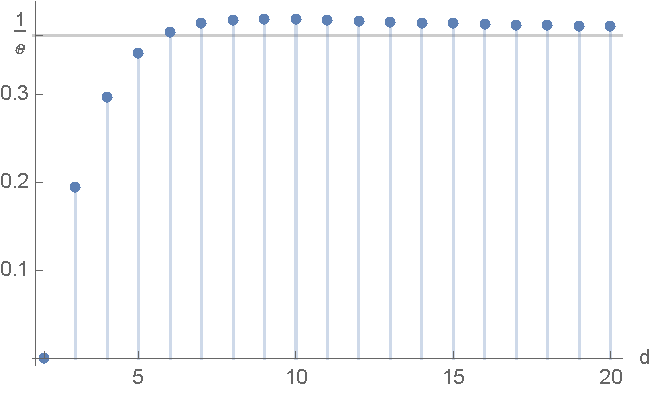
\includegraphics{boundgraph}
\caption{A chart showing the value of the bound on $q(\mathcal{G})$ for quantum-mechanically accessible $\mathcal{G}$ as a function of the Hilbert space dimension $d$.}
\label{boundgraph}
\end{center}
\end{figure}
Above, it was shown that a spherical cap taking up a proportion of $(1-\nicefrac1d)^{d-1}$ of Hilbert space must capture at least one vector from every orthonormal basis. However, if for many bases this spherical cap captures more than one basis element, this might suggest that this spherical cap was not the most efficient way of choosing a vector from each basis. We note, though, that the exact geometry of the set of projectors will have a large effect on the efficiency of inefficiency of this constructrion. It is of note that an increase in the quantum dimension, while allowing for more complicated structures and interplay of the permitted projectors that, as we shall demonstrate, seems to allow for construction of quantum graphs with very small independence number, also has a dampening affect on the quantity $|T|$ since the bases themselves have more geometrical constraints. %annulise this

We note that while a spherical cap taking up a proportion $(1-\nicefrac1d)^{d-1}$ of the Hilbert space must contain at least one out of a basis of $d$ vectors, it can actually contain up to $d$ in the worst case. Below, we will see a specific example of a set of vectors providing a nonlocality scenario, in which \emph{every} projector is captured by a pessimally-chosen spherical cap position. In $d$-dimensional Hilbert space, a spherical cap of proportion $(1-\nicefrac1n)^{d-1}$ can capture $n$ vectors out of a basis. So for any chosen $n'$, as $d$ increases, we see that the fraction of the spherical cap in the construction that cannot capture $n'$ of a basis tends to 0. However, if we consider the fraction of the spherical cap that can capture a constant proportion of basis elements $c$, we get the following behaviour under increasing $d$: %annulise this too
\begin{equation}
\lim_{d\rightarrow\infty} \left(1-\frac{1}{cd}\right)^{d-1}=e^{-\frac1c}.
\end{equation}
This might imply that the quality of the bound does not degrade as the dimension increases.%Think about this some more.


\subsection{Hadamard States and the Hadamard Graph}

In quantum dimension $d$, consider following family of states indexed by bitstrings $\vec{x}\in\{0,1\}^d$:
\begin{equation}
\mathcal{H}_d=\left\{ \ket{\psi_{\vec{x}}}:\ket{\psi_{\vec{x}}} = \frac{1}{\sqrt{d}}\sum_{i=0}^{d-1}(-1)^{x_i}\ket{i}  \right\}.
\end{equation}
These are called \emph{Hadamard states}. In dimensions $d=2^n$, they form bases which we will call \emph{Hadamard bases}. In this section, we may also consider the following set, which we will call \emph{reduced Hadamard states}.
\begin{equation}
\mathcal{R}_d=\left\{ \ket{\psi_{\vec{x}}}:\ket{\psi_{\vec{x}}} = \frac{1}{\sqrt{d}}\left(\ket{0}+\sum_{i=1}^{d-1}(-1)^{x_{i-1}}\ket{i}  \right)\right\}, \qquad\vec{x}\in\left\{\vec{x}\in\{0,1\}^{d-1}:\sum_{i=0}^{d-1} x_i =0 \enspace \mbox{mod 2}\right\}
\end{equation}
We can see that this is just the subset of Hadamard states featuring an even number of $-$ signs, with the phase degree of freedom fixed. The reason for this is computational ease; it can be easily seen that when we construct the orthogonality graph for the Hadamard states, it contains two connected components, isomorphic under the reversing the sign of any one basis element. This is because a vector with an odd number of negative components and one with an even number of negative components can never be orthogonal. Hence, all the structure captured by the Hadamard states is also captured by the set of reduced Hadamard states. We fix the phase merely so as to avoid any ambiguity of description.

The Hadamard states in dimension $d$ form what is known as the Hadamard graph. An application of the [cite] theorem tells us that we can bound the independence number of the . It's known that there exist Hadamard bases in dimensions $d=2^k$, but it is not known that Hadamard bases exist in general in all dimensions $d=4k$, suggesting that Hadamard bases have a complicated structure, and that even enumerating the Hadamard bases may not even be in \textbf{P}, since the number of vectors in our set is exponential in $d$. As such, question of what the value of $\min|T|$  is for such graphs is open and is likely to be a difficult question. The Hadamard graphs illustrate a tension in trying to optimise $q(\mathcal{G})$. They are so well connected that they have an exponentially small independence density, so few vectors can recieve a noncontextual assignment of 1, but this same connectedness means that allowing a single vector's valuation to vary contextually ``fixes'' many contexts.

\begin{figure}
\begin{center}
\begin{tabular}{|c | c | c| c|c| }\hline
Name & Transversal Size & Independence Number &FoM& Quantum? \\ \hline
\makecell{Generic Quantum\\ Graph} & $\leq\left(1-\frac1d\right)^{d-1}\leq 0.\dot{4}$ & ?&?&\ding{51} \\\hline
\makecell{$d$-Dimensional \\ Hadamard Graphs} &$\leq\frac1e$ &$\leq2de^{-cd}$&?&\ding{51} \\\hline
%\makecell{Andr\'{a}sfai\\ Graphs} & $n-\frac{n+1}{3}$ & $\frac{n+1}{3}$&$\frac{1}{3}$& \ding{55} \\\hline
\makecell{ABK Triangle-Free\\Graphs} & $n-C\sqrt{n\log n}$ & $C\sqrt{n\log n}$  & 1 &\ding{55}\\\hline
\makecell{Disjoint Graph Union of \\ small KS Graphs} &\emph{e.g.} $\frac{5n}{18}$&\emph{e.g.} $\frac{4n}{18}$& $\geq\frac{1}{18}$&\ding{51} \\ \hline
\end{tabular}
\end{center}
\caption{A table comparing the graph constructions in this paper. The quantities for the entry ``Disjoint Graph Union of small KS Graphs'' were calculated for multiple disjoint copies of Cabello's proof \cite{Cabe1997} of the Bell-Kochen-Specker theorem with 18 rays and 9 contexts.}
\end{figure}
\subsection{Triangle-Free Graphs}

Many members of the family of triangle-free graphs are not quantumly accessible. However, they do allow us to prove a concrete bound on what values of $q(\mathcal{G})$ are achievable within the framework of generalised probabilistic theories. In these graphs, the maximum cliques are merely edges, and so each context consists of two measurement objects. Quantum mechanically, the only such graphs are uninteresting: the disjoint graph union of $K_2$ graphs, and these do not have enough structure to form a proof of the Bell-Kochen-Specker theorem. In such graphs, the concept of a maximum-clique hitting-set reduces to that of to a covering of edges by vertices, a concept introduced earlier as a \emph{vertex cover}. The size of the minimal vertex cover of $\mathcal{G}$ is denoted $\tau(\mathcal{G})$. This reduction of one of our quantities of interest to one better-studied in the literature allows us to make better use of already-known results.

In the triangle-free case, we have a powerful relation between maximum-clique hitting-sets and independent sets; namely that they are graph complements of each other. A maximum-clique hitting-set, or vertex cover, is a set of vertices $T$ such that for every edge, at least one of that edge's vertices is in $T$. We can see, then, that the set $V-T$ must be independent, since if there were two vertices in $V-T$ connected by an edge, then neither of those vertices would be in $T$, a contradiction. Conversely, if we have an independent set $A$, then $V-A$ must be a vertex cover; if there were an edge with neither vertex in $V-A$, then both vertices are in $A$, a contradiction. This means that we can bound $q_a(\mathcal{G})$ as
\begin{equation}
q_a(\mathcal{G})\geq \min_\mathcal{G} |T| - \alpha(\mathcal{G}) = |V(\mathcal{G})|-2\alpha(\mathcal{G}).
\end{equation}
In other words, to be able to lower bound $q_a(\mathcal{G})$, we need only consider the independence number, $\alpha(\mathcal{G})$. We seek, therefore, triangle-free graphs with low independence number. We can invoke here a theorem due to Alon, Ben-Shimon and Krivelevich.\cite{Alon2010}
\begin{thm}
There exists a constant $C$ such that for all $n\in\mathbb{N}$ there exists a regular triangle-free graph $\mathcal{G}_n$, with $V(\mathcal{G}_n)=n$, and $\alpha(\mathcal{G}_n)\leq C\sqrt{n\log n}$.
\end{thm}

Hence, we have
\begin{align}
\lim_{n\rightarrow\infty}q(\mathcal{G}_n)&\geq\lim_{n\rightarrow\infty}\frac{n-2C\sqrt{n\log n}}{n}\\
&\geq 1-2C\lim_{n\rightarrow\infty}\sqrt{\frac{\log n}{n}}=1.
\end{align}
So, we have $q(\mathcal{G}_n)=1$ is approachable in the limit of $n\rightarrow\infty$. We see then that quantum mechanics does not display maximal contextuality as robustly, given this definition of robustness, as other possible GPTs. This could potentially have an impact on attempts to recreate quantum mechanics as a principle theory.

\FloatBarrier
\section{Classical Communication cost}

\section{Future Work}



\bibliography{/Users/andrewsimmons/Documents/Latex/Bib/bibliography}{}
\bibliographystyle{plain}

\end{document}

In which equality holds between equations \ref{eqn:1} and \ref{eqn:2} since as the indicator function for the spherical cap is twirled by the rotation group it becomes a constant function with value $p(t_1,t_2)$. Now, we would like to interpret the left hand side as an average over the elements $g\in SU(d)$ of $h(g,p,\epsilon)$, the number of the $\ket{\psi_i}$ that intersect the annulus $g^{-1}A_{t_1,t_2}$. However, we note that since the bump functions are not exact delta functions, there is by necessity some over- or under-counting of the point density, depending on whether a bump function, centred inside the annulus, has some of its measure outside the annulus; or a bump function centred outside the annulus has some of its measure within. We note that if we contract our annulus's extent by $\epsilon$, we cease to capture any of the measure of the bump functions outside the original spherical annulus. This means that the expression now represents an underestimate of the exact count of points within the annulus $g^{-1}A_{t_1,t_2}$. Contracting the annulus by $\epsilon$, so that we have $t_1\rightarrow t_1+\epsilon$ and $t_2\rightarrow t_2-\epsilon$,  has an effect on the proportion of the sphere taken up by the annulus:
\begin{align}
p(t_1+\epsilon,t_2-\epsilon)&=\left(1-t_1-\epsilon\right)^{d-1}-\left(1-t_2+\epsilon\right)^{d-1}\\
&=(1-t_1)^{d-1}-(1-t_2)^{d-1}-(d-1)\epsilon\left((1-t_1)^{d-2}+(1-t_2)^{d-2}\right)+o(\epsilon).
\end{align}
We can consider this to be a strict undercount of the true number of points within the annulus. We therefore get
\begin{equation}
q(\mathcal{G})\leq 
\end{equation}

